\documentclass[11pt, oneside]{article}   	% use "amsart" instead of "article" for AMSLaTeX format
\usepackage{geometry}                		% See geometry.pdf to learn the layout options. There are lots.
\geometry{letterpaper}                   		% ... or a4paper or a5paper or ... 
%\geometry{landscape}                		% Activate for for rotated page geometry
%\usepackage[parfill]{parskip}    		% Activate to begin paragraphs with an empty line rather than an indent
\usepackage{graphicx}				% Use pdf, png, jpg, or eps� with pdflatex; use eps in DVI mode
								% TeX will automatically convert eps --> pdf in pdflatex		
\usepackage{amssymb}
\usepackage{amsmath}
\usepackage{parskip}
\usepackage{color}
\usepackage{hyperref}

\title{Integrating zz + 1}
%\author{The Author}
%\section{}
%\subsection*{}
\date{}							% Activate to display a given date or no date

\graphicspath{{/Users/telliott_admin/Dropbox/Tex/png/}}
% \begin{center} 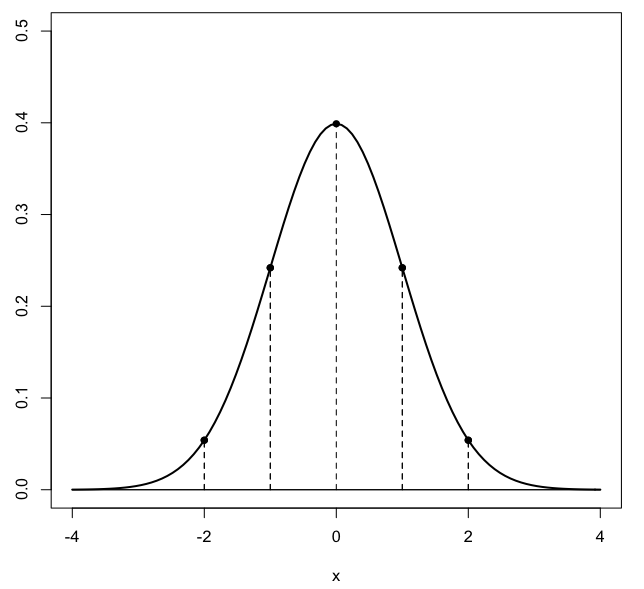
\includegraphics [scale=0.4] {gauss3.png} \end{center}
\begin{document}
\maketitle
\Large
This problem is from wikipedia.  Consider
\[ g(z) = \frac{z^2}{z^2 + 2z + 2} \]
We want to evaluate the integral:
\[ I = \oint g(z) \ dz \]
The zeroes of the denominator are
\[ \frac{-2 \pm \ \sqrt{4-8}}{2} = -1 \pm \  \frac{\sqrt{-4}}{2} = - 1 \pm \ i \]
Confirm
\[ (z + (1 - i)) \ (z + (1 + i)) \]
\[ = z^2 + z + iz + z + 1 + i -iz - i + 1 \] 
\[ = z^2 + 2z + 2 \]
The denominator can then be rewritten as
\[ = \frac{A}{z + (1 - i)} + \frac{B}{z + (1 + i)}  \]
From the numerator we have
\[ A(z + (1 + i)) + B(z + (1 - i)) = 1 \]
So $A = -B$ and
\[ A(1 + i) + B(1 - i) = 1 \]
\[ A (1 + i) - A(1 - i) = 1 \]
\[ A 2i = 1 \]
\[ A = -\frac{1}{2i}, \ \ \ B = \frac{1}{2i} \]
The integral is
\[ \oint z^2 \ [ \ \frac{-1}{2i} \ \frac{1}{z + (1 - i)} + \frac{1}{2i} \ \frac{1}{z + (1 + i)} \ ] \ dz \]
If the contour is $|z| = 2$ (the circle of radius $2$, then both of the points lie within the contour.

We have two points
\[ z = -1 - i, \ \ \ z = -1 + i \]
We evaluate $2 \pi i f(z_0)$ for each and add them, where
\[ f(z) = -\frac{z^2}{2i} \]
\[ f(z_0) = -\frac{1}{2i} \ (-1 -i)^2 = -\frac{1}{2i} \ (1 + 2i -1) = -1 \]

for the first and for the second
\[ f(z) = \frac{z^2}{2i} \]
\[ = \frac{1}{2i} \ (-1 + i)^2 = \frac{1}{2i} (1 - 2i - 1) = -1 \]
Adding them together, the answer is just $I = -2 \times 2 \pi i = - 4 \pi i $.


\end{document}  